% Copyright 2006 by Till Tantau and Mark Wibrow
%
% This file may be distributed and/or modified
%
% 1. under the LaTeX Project Public License and/or
% 2. under the GNU Free Documentation License.
%
% See the file doc/generic/pgf/licenses/LICENSE for more details.

\section{Shape Library}
\label{section-libs-shapes}

In addition to the standard shapes |rectangle|, |circle| and
|coordinate|, there exist a number of additional shapes defined in
different shape libraries. Several of these shapes have been 
contributed by Mark Wibrow. In the present section, these shapes are
described.


\begin{pgflibrary}{shapes}
  This library packages just includes all of the libraries defined in
  the following. Note that it includes only those libraries starting
  with |shapes.|, more special-purpose libraries are described in
  dedicated sections.
\end{pgflibrary}

\subsection{Rotating shape borders} \label{section-rotating shape borders}

	Some shapes (but not all), support a special kind of rotation. This 
	rotation affects only the border of a shape and is independent of the 
	node contents, but \emph{in addition} to any other transformations.
	
\begin{codeexample}[]
\begin{tikzpicture}
  [every node={dart,shape border uses incircle,inner sep=1pt,draw}]   
  \foreach \a/\b/\c in {A/0/0, B/45/0, C/0/45, D/45/45}
    \node [shape border rotate=\b, rotate=\c] at (\b/36,-\c/36) {\a};
\end{tikzpicture}
\end{codeexample}

	There are two types of rotation: restricted and unrestricted. Which 
	type of rotation is applied is determined by on how the shape border 
	is	constructed. If the shape border is contructed using an incircle, 
	that is, a circle that tightly fits the node contents (including 
	the |inner sep|), then the rotation can be unrestricted. If, however,
	the border is constructed using the natural dimensions of the node
	contents, the rotation is restricted to integer multiples of 90 
	degrees.
	
	Why should there be two kinds of rotation and border construction?
	Borders constructed using the natural dimensions of the node contents
	provide a much tighter fit to the node contents, but to maintain 
	this tight fit, the border rotation must be restricted to multiples 
	of 90 degrees. By using an incircle, unrestricted rotation is 
	possible, but the border will not make a very tight fit to the node 
	contents.
	
\begin{codeexample}[]
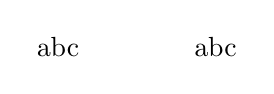
\begin{tikzpicture}[every node={isosceles triangle, draw}]
  \node {abc};
  \node [shape border uses incircle] at (2,0) {abc};
\end{tikzpicture}
\end{codeexample}

	There are \pgfname{} commands and \tikzname{} options to rotate a shape
	border and to determine how the shape border is contructed. It should
	be noted that not all shapes support these commands and options, so 
	reference should be made to the documentation for individual 
	shapes. 
	
	The \pgfname{} commands are as follows:

{\let\ifpgfshapeborderusesincircle\relax%
\begin{command}{\ifpgfshapeborderusesincircle}
   Determines if the border of a shape is constructed using an 
   incircle. 
\end{command}
}

\begin{command}{\pgfsetshapeborderrotate}
   Rotates the border of a shape independently of the node contents,
   but in addition to any other transformations. If 
   |\ifpgfshapeborderusesincircle| is false, the rotation will be
   rounded to the nearest integer multiple of 90 degrees when the
   shape is drawn. 
\end{command}

	The corresponding \tikzname{} options are:
	
\begin{itemize}

	\itemoption{shape border uses incircle}|=|\meta{true}|/|\meta{false}
	\itemoption{shape border rotate}|=|\meta{angle}
	
\end{itemize}

	It should also be noted that if the border of the shape is rotated, 
	the compass point anchors, and `text box' anchors (including 
	|mid east|, |base west|, and so on), \emph{do not rotate}, but the 
	other anchors do:
	
\begin{codeexample}[]
\begin{tikzpicture}
  [every node/.style={trapezium,draw,shape border uses incircle}]
  \node at (0,0)  (A) {\Large A};
  \node [shape border rotate=30] at (1.5,0) (B) {\Large B};
  \foreach \s/\t in 
    {left side/base east, bottom side/north, bottom left corner/base}{
       \fill[red]  (A.\s) circle(1.5pt) (B.\s) circle(1.5pt);
       \fill[blue] (A.\t) circle(1.5pt) (B.\t) circle(1.5pt);
  }
\end{tikzpicture}
\end{codeexample}


\subsection{Predefined Shapes}
\label{section-predefined-shapes}

The three shapes |rectangle|, |circle|, and |coordiante| are always
defined and no library needs to be loaded for them. while the
|coordinate| shape defines only the |center| anchor, the other two
shapes define a standard set of anchors.

\begin{shape}{circle}
  This shape draws a tightly fitting circle around the text. The
  following figure shows the anchors this shape defines; the anchors
  |10| and |130| are example of border anchors. 
\begin{codeexample}[]
\Huge
\begin{tikzpicture}
  \node[name=s,shape=circle,shape example] {Circle\vrule width 1pt height 2cm};
  \foreach \anchor/\placement in
    {north west/above left, north/above, north east/above right, 
     west/left, center/above, east/right, 
     mid west/right, mid/above, mid east/left, 
     base west/left, base/below, base east/right, 
     south west/below left, south/below, south east/below right, 
     text/left, 10/right, 130/above}
     \draw[shift=(s.\anchor)] plot[mark=x] coordinates{(0,0)}
       node[\placement] {\scriptsize\texttt{(s.\anchor)}};
\end{tikzpicture}
\end{codeexample}
\end{shape}

\begin{shape}{rectangle}
  This shape, which is the standard, is a rectangle around the
  text. The inner   and outer separations (see
  Section~\ref{section-shape-seps}) influence the white space around
  the text. The following figure shows the anchors this
  shape defines; the anchors |10| and |130| are example of border anchors.
\begin{codeexample}[]
\Huge
\begin{tikzpicture}
  \node[name=s,shape=rectangle,shape example] {Rectangle\vrule width 1pt height 2cm};
  \foreach \anchor/\placement in
    {north west/above left, north/above, north east/above right, 
     west/left, center/above, east/right, 
     mid west/right, mid/above, mid east/left, 
     base west/left, base/below, base east/right, 
     south west/below left, south/below, south east/below right, 
     text/left, 10/right, 130/above}
     \draw[shift=(s.\anchor)] plot[mark=x] coordinates{(0,0)}
       node[\placement] {\scriptsize\texttt{(s.\anchor)}};
\end{tikzpicture}
\end{codeexample}
\end{shape}


\subsection{Geometric Shapes}

\begin{pgflibrary}{shapes.geometric}
  This library defines different shapes that correspond to basic
  geometric objects like ellipses or polygons.
\end{pgflibrary}



\begin{shape}{diamond}
  This shape is a diamond tightly fitting the text box. The ratio
  between width and height is 1 by default, but can be changed by
  setting the shape aspect ratio (using the following command or the
  |aspect| option of \tikzname). The following figure shows the anchors this
  shape defines; the anchors |10| and |130| are example of border
  anchors.

  \begin{command}{\pgfsetshapeaspect\marg{value}}
    This command sets the macro \declare{|\pgfshapeaspect|} to
    \meta{value}. Furthermore, \declare{|\pgfshapeaspectinverse|} is set
    to the reciprocal of \meta{value}. The aspect is a recommendation
    for the quotient of the width and the height of a shape.
  \end{command}

\begin{codeexample}[]
\Huge
\begin{tikzpicture}
  \node[name=s,shape=diamond,shape example] {Diamond\vrule width 1pt height 2cm};
  \foreach \anchor/\placement in
    {north west/above left, north/above, north east/above right, 
     west/left, center/above, east/right, 
     mid/above, 
     base/below,  
     south west/below left, south/below, south east/below right, 
     text/left, 10/right, 130/above}
     \draw[shift=(s.\anchor)] plot[mark=x] coordinates{(0,0)}
       node[\placement] {\scriptsize\texttt{(s.\anchor)}};
\end{tikzpicture}
\end{codeexample}
\end{shape}

\begin{shape}{ellipse}
  This shape is an ellipse tightly fitting the text box, if no inner
  separation is given. The following figure shows the anchors this
  shape defines; the anchors |10| and |130| are example of border anchors.
\begin{codeexample}[]
\Huge
\begin{tikzpicture}
  \node[name=s,shape=ellipse,shape example] {Ellipse\vrule width 1pt height 2cm};
  \foreach \anchor/\placement in
    {north west/above left, north/above, north east/above right, 
     west/left, center/above, east/right, 
     mid west/right, mid/above, mid east/left, 
     base west/left, base/below, base east/right, 
     south west/below left, south/below, south east/below right, 
     text/left, 10/right, 130/above}
     \draw[shift=(s.\anchor)] plot[mark=x] coordinates{(0,0)}
       node[\placement] {\scriptsize\texttt{(s.\anchor)}};
\end{tikzpicture}
\end{codeexample}
\end{shape}





\begin{shape}{trapezium}
	This shape is a trapezium, that is, a quadrilateral with a single
	pair of parallel lines (this can sometimes be known as a trapezoid).
	The |trapezium| shape supports the rotation of the shape border, as 
	described in Section~\ref{section-rotating shape borders}. 
   
   By default, the the lower corners of the trapezium are extended 
	(i.e., `stick out') by a distance of 1.5ex, but each can be extended 
	independently.	

	
\begin{codeexample}[]
\begin{tikzpicture}[every node/.style={trapezium, draw}]
   \node at (0,1) {A};
   \node[trapezium left extension=10pt, trapezium right extension=20pt]
         at (0,0) {B};
\end{tikzpicture}
\end{codeexample}

   Negative extensions result in the upper points being extended. This
   means that parallelograms can be created (but technically these are
   not trapezia, as they have more than one pair of parallel sides).
   These extensions are in addition to the natural dimensions of the
   node contents.
   
\begin{codeexample}[]
\begin{tikzpicture}[every node/.style={trapezium, draw}]
   \node[trapezium left extension=10pt, trapezium right extension=20pt]
         at (0,2) {A};
   \node[trapezium left extension=-10pt, trapezium right extension=-20pt]
         at (0,1) {B};
   \node[trapezium left extension=-10pt, trapezium right extension=10pt]
         at (0,0) {C};
\end{tikzpicture}
\end{codeexample}

	There are \pgfname{} commands and \tikzname{} options to set the 
  	extensions of the trapezium. The \pgfname{} commands are as follows:
	
	\begin{command}{\pgftrapeziumleftextension\marg{length}}
    Set the distance that the lower left corner `sticks out'. If 
    \meta{length} is negative, the upper left corner is adjusted.
   \end{command}
   
   \begin{command}{\pgftrapeziumrightextension\marg{length}}
    Set the distance that the lower right corner `sticks out'. If 
    \meta{length} is negative, the upper right corner is adjusted.
   \end{command}
   
   The corresponding \tikzname{} options are:

  \begin{itemize}
    \itemoption{trapezium left extension}|=|\meta{length}
    set the extension for the lower left corner (negative values adjust
    the upper left corner).
    
    \itemoption{trapezium right extension}|=|\meta{length}
    set the extension for the lower right corner (negative values adjust
    the upper right corner).
    
    \itemoption{trapezium extension}|=|\meta{length}
    set the extension for both lower corners (negative values adjust
    the upper corners).
    
  \end{itemize}
  
   The anchors for the trapezium are shown below. The anchor |150| is an
	example of a border anchor.

\begin{codeexample}[]
\Huge
\begin{tikzpicture}
  \node[name=s, shape=trapezium, trapezium extension=2cm, shape example, inner sep=1.5cm] 
    {Trapezium\vrule width 1pt height 2cm};
  \foreach \anchor/\placement in
    {bottom left corner/below, top right corner/right, 
     top left corner/left,     bottom right corner/below,
     bottom side/below,        left side/left, 
     right side/right,         top side/above,
     center/above,   text/below,      mid/right,       base/below, 
     mid west/right, base west/below, mid east/left,   base east/below, 
     west/above,     east/above,      north/below,     south/above,
     north west/above, north east/above, 
     south west/below, south east/below, 150/above}    
  \draw[shift=(s.\anchor)] plot[mark=x] coordinates{(0,0)}
    node[\placement] {\scriptsize\texttt{(s.\anchor)}};
\end{tikzpicture}
\end{codeexample}  
   
\end{shape}





\begin{shape}{semicircle}
	
	This shape is a semicircle, which tightly fits the node contents.
	This shape supports the rotation of the shape border, as described in 
	Section~\ref{section-rotating shape borders}.
	The anchors for the |semicircle| shape are shown below. 
	Anchor |30| is an example of a border anchor.
	
\begin{codeexample}[]
\Huge
\begin{tikzpicture}
  \node[name=s,shape=semicircle,shape border rotate=0,shape example, inner sep=1cm] 
  	{Semicircle\vrule width 1pt height 2cm};
  \foreach \anchor/\placement in
    {apex/above,      arc start/below, arc end/below,  chord center/below,
     center/above,    base/below,      mid/right,      text/left,
     base west/below, base east/below, mid west/left, mid east/right, 
     north/below,     south/above,     east/above,     west/above,
     north west/above left, north east/above right,
     south west/below,      south east/below, 30/right}
     \draw[shift=(s.\anchor)] plot[mark=x] coordinates{(0,0)}
       node[\placement] {\scriptsize\texttt{(s.\anchor)}};
\end{tikzpicture}
\end{codeexample}
\end{shape}





\begin{shape}{regular polygon}
  This shape is a regular polygon, which, by default, is drawn so that 
  a side (rather than a corner) is always at the bottom. 
  This shape supports the rotation as described in 
  Section~\ref{section-rotating shape borders}, but the border of the 
  polygon is \emph{always} constructed using the incircle, whose
  radius is calculated to tightly fit the node contents. (including
  any |inner sep|).
  
\begin{codeexample}[]
\begin{tikzpicture}
  \foreach \a in {3,...,7}{
    \draw[gray!50] (\a*2,0)  circle(0.5cm);
    \node[regular polygon, regular polygon sides=\a,
          inner sep=0cm, text=red!50, draw] 
          at (\a*2,0) {\vrule height 0.707cm width 0.707cm};
   }  
\end{tikzpicture}
\end{codeexample}	
	
  If the node is enlarged to any specified minimum size, 
  this is interpreted as the diameter of the the 
  circumcircle, that is, the circle that passes through all the 
  corners of the polygon border.

\begin{codeexample}[]
\begin{tikzpicture}
  \foreach \a in {3,...,7}{
    \draw[gray!50] (\a*2,0)  circle(0.5cm);
    \node[regular polygon, regular polygon sides=\a, minimum size=1cm, draw] at (\a*2,0) {};
   }  
\end{tikzpicture}
\end{codeexample}	

  There is a \pgfname{} command and \tikzname{} option to set the 
  number of sides for the polygon. The \pgfname{} command is as 
  follows:
	
  \begin{command}{\pgfsetpolygonsides\marg{integer}}
  \end{command}
  
  The corresponding \tikzname{} option is:

  \begin{itemize}
    \itemoption{regular polygon sides}|=|\meta{integer}
  \end{itemize}
  
  The anchors for the regular polygon shape are shown below.  
  The anchor |75| is an example of a border anchor.
  
\begin{codeexample}[]
\Huge
\begin{tikzpicture}
  \node[name=s, shape=regular polygon, regular polygon sides=5, shape example, inner sep=.5cm] 
    {Regular Polygon\vrule width 1pt height 2cm};
  \foreach \anchor/\placement in
    {corner 1/above, corner 2/above, corner 3/left, corner 4/right, corner 5/above, 
     side 1/above,   side 2/left,    side 3/below,  side 4/right,   side 5/above,  
     center/above, text/left,  mid/right,   base/below, 75/above,
     west/above,   east/above, north/below, south/above,
     north east/below, south east/above, north west/below, south west/above}
  \draw[shift=(s.\anchor)] plot[mark=x] coordinates{(0,0)}
    node[\placement] {\scriptsize\texttt{(s.\anchor)}};
\end{tikzpicture}
\end{codeexample}

\end{shape}

\begin{shape}{star}
  This shape is a star, which by default (minus any transformations) is
  drawn with the first point pointing upwards.  
  This shape supports the rotation as described in 
  Section~\ref{section-rotating shape borders}, but the border of the 
  star is \emph{always} constructed using the incircle.
  
  A star should be thought of as having an set of ``inner points'' and
  and ``outer points''. 
  The inner points of the border are based on the radius of the circle
  which tightly fits the node contents, and the outer points are based
  on the circumcircle, the circle that passes through every outer
  point.
  Any specified minimum size, width or height, is interpreted as the 
  diameter of the circumcircle.
 
\begin{codeexample}[]
\begin{tikzpicture}
   \draw [help lines]   (0,0) grid (2,2);
   \draw [red, dashed]  (1,1) circle(1cm);
   \draw [blue, dashed] (1,1) circle(.5cm);
   \node [star, star point height=.5cm, minimum size=2cm, draw] 
       at (1,1) {S};
\end{tikzpicture}
\end{codeexample} 
  
  There are \pgfname{} commands and \tikzname{} options to set the 
  number of points, and the height of the star points.
  The \pgfname{} commands are as follows:
  
  \begin{command}{\pgfsetstarpoints\marg{integer}}
    Sets the number of points for the star.
  \end{command}
  
  \begin{command}{\pgfsetstarpointheight\marg{distance}}
    Sets the height of the star points. This is the distance between the
    inner point and outer point radii. If the star is enlarged to some
    specified minimum size, the inner radius is increased to maintain
    the point height.	
  \end{command}
  
  \begin{command}{\pgfsetstarpointratio\marg{number}}
    Sets the ratio between the inner point and outer point radii.		
    If the star is enlarged to some specified minimum size, the
    inner radius is increased to maintain the ratio.	
  \end{command}
  
  The corresponding \tikzname{} options are:
  
  \begin{itemize}
    \itemoption{star points}|=|\meta{integer}
    set the number of points for the star.
    
    \itemoption{star point height}|=|\meta{distance}
    set the height of the points for the star.
    
    \itemoption{star point ratio}|=|\meta{number}
    set the ratio between the outer point radius and the inner point
    radius.
    
  \end{itemize}

	The inner and outer points form the principle anchors for the star,
   as shown below (anchor |75| is an example of a border anchor).
  
  \begin{codeexample}[]
\Huge
\begin{tikzpicture}
  \node[name=s, shape=star, star points=5, star point ratio=1.65, shape example, inner sep=1.5cm] 
    {Star\vrule width 1pt height 2cm};
  \foreach \anchor/\placement in
     {inner point 1/above, inner point 2/above, inner point 3/below, inner point 4/right, 
      inner point 5/above, outer point 1/above, outer point 2/above, outer point 3/left,  
      outer point 4/right, outer point 5/above,
      center/above, text/left,  mid/right,   base/below, 75/above,
     	west/above,   east/above, north/below, south/above,
     	north east/below, south east/above, north west/below, south west/above}
  \draw[shift=(s.\anchor)] plot[mark=x] coordinates{(0,0)}
    node[\placement] {\scriptsize\texttt{(s.\anchor)}};
\end{tikzpicture}
\end{codeexample}
\end{shape}





\begin{shape}{isosceles triangle}
	This shape is an isosceles triangle, which supports the rotation of 
	the shape border, as described in 
	Section~\ref{section-rotating shape borders}.
	
	Minimum size and minimum width requirements ensure the literal width 
	and height of the isosceles triangle, but are applied as if the 
	triangle is rotated to 90 degrees (i.e., with the apex pointing up). 
	In order to keep the apex angle the same, increasing the height will 
	increase the width and vice versa. 
   
\begin{codeexample}[]
\begin{tikzpicture}
  [every node/.style={
    isosceles triangle,
    draw,
    inner sep=0pt, 
    anchor=left corner,
    shape border rotate=90}]
   \draw[help lines] grid(4,2);
   \foreach \a/\c in {1.5/blue, 1/green, 0.5/red}{
      \color{\c}
      \node[minimum height=\a cm] at (0,0) {};
      \node[minimum width=\a cm] at (2,0) {};
   }
\end{tikzpicture}
\end{codeexample}	

	There is a \pgfname{} command and \tikzname{} option to set the 
  	apex angle of the triangle. The \pgfname{} command is as follows:
    
  \begin{command}{\pgfsetisoscelestriangleapexangle\marg{angle}}
    Sets the angle of the apex of the isosceles triangle. The height
    and width of the triangle may be adjusted to maintain this
    angle.
  \end{command}
  
  The \tikzname{} option is:
  
  \begin{itemize}
    \itemoption{isosceles triangle apex angle}|=|\meta{angle}
    set the angle of the apex of the isosceles triangle.
   \end{itemize}
 
	The anchors for the |isosceles triangle| are shown below (the border 
	has been rotated 90 degrees anticlockwise). Anchor |150| is an
	example of a border anchor. 
\begin{codeexample}[]
\Huge
\begin{tikzpicture}
  \node[name=s, shape=isosceles triangle, shape border uses incircle, shape example, 
        shape border rotate=90, inner sep=0cm] 
    {Isosceles Triangle\vrule width 1pt height 2cm};
  \foreach \anchor/\placement in
    {apex/above,      left corner/above right, right corner/above left,
     left side/above, right side/above,        lower side/below,    
     center/above,  text/left,       mid/right,      base/below, 
     mid west/left, base west/below, mid east/right, base east/below,
     west/above,    east/above,      north/below,    south/above,
     north west/left,  north east/right, 
     south west/below, south east/below, 150/above}  
  \draw[shift=(s.\anchor)] plot[mark=x] coordinates{(0,0)}
    node[\placement] {\scriptsize\texttt{(s.\anchor)}};
\end{tikzpicture}
\end{codeexample} 

\end{shape}


\par\leavevmode
\begin{shape}{kite}

	This shape is a kite, which supports the rotation of the shape border, 
	as described in Section~\ref{section-rotating shape borders}. 
	There are \pgfname{} commands and \tikzname{} 
	options to specify the upper and lower	vertex angles of the kite. 
	The \pgfname{} commands are as follows:
	
	\begin{command}{\pgfsetkiteuppervertexangle\marg{angle}}
	Set the upper internal angle of the kite.
	\end{command}
	
	\begin{command}{\pgfsetkitelowervertexangle\marg{angle}}
	Set the lower internal angle of the kite.
	\end{command}
	
	The corresponding \tikzname{} options are as follows:
	
	\begin{itemize}
    \itemoption{kite upper vertex angle}|=|\meta{integer}
    \itemoption{kite lower vertex angle}|=|\meta{angle}
    \itemoption{kite vertex angles}|={|\meta{angle specification}|}|
    
    \meta{angle specification} can be a comma separated pair 
    |{|\meta{upper angle}|,|\meta{lower angle}|}|, or a single angle.
    In this latter case, both the upper and lower vertex angles will 
    be the same (and in addition, the braces |{}| can be omitted).
    
\begin{codeexample}[]
\begin{tikzpicture}[every node/.style={kite, draw}]
  \node[kite upper vertex angle=135, kite lower vertex angle=70] at (0,0) {A};
  \node[kite vertex angles={90,45}] at (1,0) {B};
  \node[kite vertex angles=60]      at (2,0) {C};
\end{tikzpicture}
\end{codeexample}

 \end{itemize}

	The anchors for the |kite| are shown below. Anchor |110| is an 
	example of a border anchor.
	
\begin{codeexample}[]
\Huge
\begin{tikzpicture}
  \node[name=s, shape=kite, shape example, inner sep=1.5cm] 
    {Kite\vrule width 1pt height 2cm};
  \foreach \anchor/\placement in
    {upper vertex/above, left vertex/above,    lower vertex/below, 
     right vertex/above, upper left side/above, upper right side/above,
     lower left side/below, lower right side/below,
     center/above,   text/left,       mid/right,        base/below, 
     mid west/left,  base west/below, mid east/right,   base east/below,
     west/above,     east/above,      north/below,     south/above,
     north west/left, north east/right, 
     south west/above, south east/above, 110/above}  
  \draw[shift=(s.\anchor)] plot[mark=x] coordinates{(0,0)}
    node[\placement] {\scriptsize\texttt{(s.\anchor)}};
\end{tikzpicture}
\end{codeexample}
\end{shape}


\begin{shape}{dart}


	This shape is a dart (which can also be known as an arrowhead or
	concave kite). This shape supports the rotation of the shape border, 
	as described in Section~\ref{section-rotating shape borders}. 
	The angle of the border rotation determines the direction in which 
	the dart points (unless other transformations have been applied).
	
	There are \pgfname{} commands and \tikzname{} options, to set the 
	angle for the `tip' of the dart and the angle between the `tails'
	of the dart. These angles default to 45 degrees and 135 degrees 
	respectively.

\begin{codeexample}[]
\begin{tikzpicture}
   \node[dart, draw, gray, shape border uses incircle, shape border rotate=45] 
       (d) {dart};
   \draw [<->] (d.tip)++(202.5:.5cm) arc(202.5:247.5:.5cm);
   \node [left of=.5cm] at (d.tip) {tip angle};
   \draw [<->] (d.tail center)++(157.5:.5cm) arc(157.5:292.5:.5cm);
   \node [right] at (d.tail center) {tail angle};
\end{tikzpicture}
\end{codeexample}

	The \pgfname{} commands are as follows:
	
	\begin{command}{\pgfsetdarttipangle\marg{angle}}
		Set the angle at the tip of the dart.
	\end{command}
	
	\begin{command}{\pgfsetdarttailangle\marg{angle}}
		Set the angle between the tails of the dart.
	\end{command}
	
	The corresponding \tikzname{} options are:
	
	\begin{itemize}
		\itemoption{dart tip angle}|=|\meta{angle}
		
		\itemoption{dart tail angle}|=|\meta{angle}		
	\end{itemize}
	
	The anchors for the |dart| shape are shown below (note that the 
	shape is rotated 90 degrees anti-clockwise). Anchor |110| is an 
	example of a border anchor.
\begin{codeexample}[]
\Huge
\begin{tikzpicture}
  \node[name=s, shape=dart, shape border rotate=90, shape example, inner sep=1.25cm] 
    {Dart\vrule width 1pt height 2cm};
  \foreach \anchor/\placement in
    {tip/above,       tail center/below, right tail/below, 
     left tail/below, right tail/below,  left side/left,   right side/right,
     center/above,    text/left,         mid/right,        base/below, 
     mid west/left,   base west/below,   mid east/right,   base east/below,
     west/above,      east/above,        north/below,      south/above,
     north west/left, north east/right,  south west/above, south east/above,
     110/above}    
  \draw[shift=(s.\anchor)] plot[mark=x] coordinates{(0,0)}
    node[\placement] {\scriptsize\texttt{(s.\anchor)}};
\end{tikzpicture}
\end{codeexample}
\end{shape}




\begin{shape}{circular sector}

	This shape is a circular sector (which can also be known as a
	wedge).
	This shape supports the rotation of the shape border, 
	as described in Section~\ref{section-rotating shape borders}. 
	The angle of the border rotation determines the direction in which 
	the `apex' of the sector points (unless other transformations have 
	been applied).
	
\begin{codeexample}[]
\begin{tikzpicture}
  [every node/.style={circular sector, shape border uses incircle, draw}]
  \node at (0,0) {A};
  \node [shape border rotate=30] at (1.5,0) {A};
\end{tikzpicture}
\end{codeexample}

	There is a \pgfname{} command and \tikzname{} option to set the 
	central angle of the sector, which is expected to be less than 180
	degrees. This central angle defaults to 60 degrees.
	
	\begin{command}{\pgfsetcircularsectorangle\marg{angle}}
		Set the central angle of the sector. 
	\end{command}
	
	The corresponding \tikzname{} option is:
	
	\begin{itemize}
		\itemoption{circular sector angle}|=|\meta{angle}		
	\end{itemize}
	
	The anchors for the |circular sector| shape are shown below.
	Anchor |30| is an example of a border anchor.
	
\begin{codeexample}[]
\Huge
\begin{tikzpicture}
  \node[name=s,shape=circular sector,  style=shape example, inner sep=1cm] 
  	{Circular Sector\vrule width 1pt height 2cm};
  \foreach \anchor/\placement in
   {sector center/above, arc start/below, arc end/below, arc center/below,
    center/above,        base/below,      mid/right,     text/below,
    north/below,         south/above,     east/below,    west/above,
    north west/above left, north east/above right,
    south west/below,      south east/below, 30/right}
     \draw[shift=(s.\anchor)] plot[mark=x] coordinates{(0,0)}
       node[\placement] {\scriptsize\texttt{(s.\anchor)}};
\end{tikzpicture}
\end{codeexample}
\end{shape}





\subsection{Symbol Shapes}

\begin{pgflibrary}{shapes.symbols}
  This library defines shapes that can be used for drawing symbols
  like a forbidden sign or a cloud.
\end{pgflibrary}



\begin{shape}{forbidden sign}
  This shape places the node inside a circle with a diagonal from the
  lower left to the upper right added. The circle is part of the
  background, the diagonal line part of the foreground path; thus, the
  diagonal line is on top of the text.
  
\begin{codeexample}[]
\begin{tikzpicture}
  \node [forbidden sign,line width=1ex,draw=red,fill=white] {Smoking};
\end{tikzpicture}
\end{codeexample}

  The shape inherits all anchors from the |circle| shape, see also the
  following figure:
\begin{codeexample}[]
\Huge
\begin{tikzpicture}
  \node[name=s,shape=forbidden sign,shape example] {Forbidden\vrule width 1pt height 2cm};
  \foreach \anchor/\placement in
    {north west/above left, north/above, north east/above right, 
     west/left, center/above, east/right, 
     mid west/right, mid/above, mid east/left, 
     base west/left, base/below, base east/right, 
     south west/below left, south/below, south east/below right, 
     text/left, 10/right, 130/above}
     \draw[shift=(s.\anchor)] plot[mark=x] coordinates{(0,0)}
       node[\placement] {\scriptsize\texttt{(s.\anchor)}};
\end{tikzpicture}
\end{codeexample}
\end{shape}



\subsection{Shapes with Multiple Text Parts}

\begin{pgflibrary}{shapes.multipart}
  This library defines general-purpose shapes that are composed of
  multiple (text) parts. 
\end{pgflibrary}


\begin{shape}{circle split}
  This shape is a multi-part shape consisting of a circle with a line
  in the middle. The upper part is the main part (the |text| part),
  the lower part is the |lower| part.
  
\begin{codeexample}[]
\begin{tikzpicture}
  \node [circle split,draw,double,fill=red!20]
  {
    $q_1$
    \nodepart{lower}
    $00$
  };
\end{tikzpicture}
\end{codeexample}

  The shape inherits all anchors from the |circle| shape and defines
  the |lower| anchor in addition. See also the
  following figure:
\begin{codeexample}[]
\Huge
\begin{tikzpicture}
  \node[name=s,shape=circle split,shape example] {text\nodepart{lower}lower};
  \foreach \anchor/\placement in
    {north west/above left, north/above, north east/above right, 
     west/left, center/below, east/right, 
     mid west/right, mid/above, mid east/left, 
     base west/left, base/below, base east/right, 
     south west/below left, south/below, south east/below right, 
     text/left, lower/left, 130/above}
     \draw[shift=(s.\anchor)] plot[mark=x] coordinates{(0,0)}
       node[\placement] {\scriptsize\texttt{(s.\anchor)}};
\end{tikzpicture}
\end{codeexample}
\end{shape}


\subsection{Miscellaneous Shapes}

\begin{pgflibrary}{shapes.misc}
  This library defines general-purpose shapes that do not fit in the
  previous categories.
\end{pgflibrary}



\begin{shape}{cross out}
  This shape ``crosses out'' the node. Its foreground path are simply
  two diagonal lines that between the corners of the node's bounding
  box. Here is an example:

\begin{codeexample}[]
\begin{tikzpicture}
  \draw[help lines] (0,0) grid (3,2);
  \node [cross out,draw=red] at (1.5,1) {cross out};
\end{tikzpicture}
\end{codeexample}

  A useful application is inside text as in the following example:
\begin{codeexample}[]
Cross \tikz[baseline] \node [cross out,draw,anchor=text] {me}; out!  
\end{codeexample}

  This shape inherits all anchors from the |rectangle| shape, see also
  the following figure:
\begin{codeexample}[]
\Huge
\begin{tikzpicture}
  \node[name=s,shape=cross out,shape example] {cross out\vrule width 1pt height 2cm};
  \foreach \anchor/\placement in
    {north west/above left, north/above, north east/above right, 
     west/left, center/above, east/right, 
     mid west/right, mid/above, mid east/left, 
     base west/left, base/below, base east/right, 
     south west/below left, south/below, south east/below right, 
     text/left, 10/right, 130/above}
     \draw[shift=(s.\anchor)] plot[mark=x] coordinates{(0,0)}
       node[\placement] {\scriptsize\texttt{(s.\anchor)}};
\end{tikzpicture}
\end{codeexample}
\end{shape}

\begin{shape}{strike out}
  This shape is idential to the |cross out| shape, only its foreground
  path consists of a single line from the lower left to the upper
  right.
  
\begin{codeexample}[]
Strike \tikz[baseline] \node [strike out,draw,anchor=text] {me}; out!  
\end{codeexample}

  See the |cross out| shape for the anchors.
\end{shape}



%%% Local Variables: 
%%% mode: latex
%%% TeX-master: "pgfmanual-pdftex-version"
%%% End: 
